% !TEX TS-program = pdflatex
% !TEX encoding = UTF-8 Unicode

	\documentclass[11pt]{article}%                                                use larger type; default would be 10pt
\usepackage[utf8]{inputenc}%                                                      set input encoding (not needed with XeLaTeX)

%%% PAGE DIMENSIONS ------------------------------------------------------------
\usepackage[top=0.8in, left=1in, right=1in, bottom=0.8in]{geometry}%              to change the page dimensions
\geometry{a4paper}%                                                               or letterpaper (US) or a5paper or....
\usepackage[parfill]{parskip}%                                                    Activate to begin paragraphs with an empty line rather than an indent

%%% HEADERS & FOOTERS ----------------------------------------------------------
\usepackage{fancyhdr}%                                                            This should be set AFTER setting up the page geometry
\pagestyle{fancy}%                                                                options: empty , plain , fancy
\renewcommand{\headrulewidth}{0pt}%                                               customise the layout...
\lhead{}\chead{}\rhead{}
\lfoot{}\cfoot{page \thepage}\rfoot{}

%%% SECTION TITLE APPEARANCE ---------------------------------------------------
\usepackage{sectsty}
\allsectionsfont{\sffamily\mdseries\upshape}%                                     (See the fntguide.pdf for font help)

%%% PACKAGES -------------------------------------------------------------------
\usepackage[font=small,labelfont=bf,textfont=it]{caption}%                        stylize captions
\usepackage{graphicx}%                                                            support the \includegraphics command and options
\usepackage{booktabs}%                                                            for much better looking tables
\usepackage{array}%                                                               for better arrays (eg matrices) in maths
\usepackage{paralist}%                                                            very flexible & customisable lists (eg. enumerate/itemize, etc.)
\usepackage{verbatim}%                                                            adds environment for commenting out blocks of text & for better verbatim
\usepackage{subfig}%                                                              make it possible to include more than one captioned figure/table in a single float
\usepackage{mathtools}%                                                           for math environments like align
\usepackage{amssymb}%                                                             for symbols like \therefore
\usepackage{verbatim}%                                                            for including text as appears, verbatim
\usepackage{listings}%                                                            for including external files as text, eg code
\usepackage{color}%                                                               for coloring of files and images
\usepackage{overpic}%                                                             for adding annotations to pictures
	\usepackage{siunitx}
	\usepackage{multirow}

%%% EQUATIONS ------------------------------------------------------------------
\numberwithin{equation}{section}%                                                 Number equations by section (change for different levels)
	\DeclareSIUnit[number-unit-product = {}]\pixel{\text{pix}}
	\DeclareSIUnit[number-unit-product = {}]\ADU{\text{ADU}}
	\DeclareSIUnit[number-unit-product = {}]\electron{\text{e}^{-{}}}

%% BIBIOGRAPHY ------------------------------------------------------------------
\usepackage{cite}

%%% ToC (table of contents) APPEARANCE -----------------------------------------
%\usepackage[nottoc,notlof,notlot]{tocbibind}                                   % Put the bibliography in the ToC
%\usepackage[titles,subfigure]{tocloft}                                         % Alter the style of the Table of Contents
%\renewcommand{\cftsecfont}{\rmfamily\mdseries\upshape}
%\renewcommand{\cftsecpagefont}{\rmfamily\mdseries\upshape}                     % No bold!

%%% PDF LINKS AND STYLE --------------------------------------------------------
\usepackage[unicode=true,
    bookmarks=true,bookmarksnumbered=true,bookmarksopen=true,
    bookmarksopenlevel=2, breaklinks=false,pdfborder={0 0 0},backref=false,
    colorlinks=false] {hyperref}%                                                 for links in pdf file, no colors
\hypersetup{pdftitle={Cosmic Re-ionisation},
    pdfauthor={Extragalactic Astrophysics and Cosmology Group Studies}}%		  set name of document and author here

%%% END Article customizations

%%% NEW COMMANDS ---------------------------------------------------------------
\renewcommand{\d}{\,\mathrm{d}}%                                                  for integrals
\newcommand{\dx}[2]{\frac{\textrm{d}#1}{\textrm{d}#2}}%                         for derivatives
\newcommand{\dd}[2]{\frac{\textrm{d}^2#1}{\textrm{d}#2^2}}%                     for double derivatives
\newcommand{\pd}[2]{\frac{\partial#1}{\partial#2}}%                             for partial derivatives
\newcommand{\pdd}[2]{\frac{\partial^2#1}{\partial#2^2}}%                        for double partial derivatives
\newcommand{\e}[1]{\text{e}^{#1}}%                                                for exponentials
\newcommand{\code}[1]{\texttt{#1}}%                                               for verbatim code view
\newcommand{\inter}[1]{\shortintertext{#1}}%                                      shorter version of intertext
\newcommand{\under}[1]{\underline{#1}}%                                           for vectors etc.

\let\vaccent=\v{}%                                                                  rename builtin command \v{} to \vaccent{}
\newcommand{\uv}[1]{\ensuremath{\hat{#1}}}%                                       for unit vector
\newcommand{\abs}[1]{\left|#1\right|}%                                          for absolute value
\newcommand{\avg}[1]{\left<#1\right>}%                                          for average
\let\underdot=\d%                                                                 rename builtin command \d{} to \underdot{}
\newcommand{\ket}[1]{\left|#1\right>}%                                          for Dirac bras
\newcommand{\bra}[1]{\left<#1\right|}%                                          for Dirac kets
\newcommand{\braket}[2]{\left<#1\vphantom{#2} \right|
    \left.#2 \vphantom{#1} \right>}%                                             for Dirac brackets
\newcommand{\matrixel}[3]{\left<#1\vphantom{#2#3} \right|
    #2 \left|#3 \vphantom{#1#2}\right>}%                                        for Dirac matrix elements
\newcommand{\grad}[1]{\nabla#1}%                                                 for gradient
\let\divsymb=\div%                                                                rename builtin command \div to \divsymb
\renewcommand{\div}[1]{\nabla\cdot#1}%                                          for divergence
\newcommand{\curl}[1]{\nabla\times#1}%                                          for curl
\let\baraccent=\={}%                                                                rename builtin command \= to \baraccent
\renewcommand{\=}[1]{\stackrel{#1}{=}}%                                           for putting numbers above =


%*******************************************************************************
%******************************** END HEADER ***********************************
%*******************************************************************************

\begin{document}
%!TEX root = mainfile.tex
\begin{titlepage}
  \begin{center}
    \vspace*{\fill}

    \centering
    
\includegraphics[scale=1.0]{Logo.pdf}
    \vfill

    \hrule
    {\LARGE\bf Extragalactic Astrophysics and Cosmology\\Cosmic Reionization \\[0.4cm]}
    \hrule

    \vfill
    \large
    School of Physics and Astronomy\\
    University of Birmingham

    \vfill
    { Joe Baumber,
    	James Bryant,
    	Lewis Clegg,
    	Bethany Johnson,
    	Andrew King,
    	Owen McConnell,
    	Catherine McDonald,
    	Michael O'Neill,
    	Jonathan Shepley,
    	Dorothy Stonell,
    	Rahim Topadar,
    	Josh Wainwright\\}
    \vfill

    \vfill
    \textit{Supervisors:} Graham Smith, Alistair Sanderson, Melissa Gillone \\
    		\vfill
    \textit{Date:} March 2013
    \vfill
    \vfill

    \begin{abstract}
        This study deduces that reionization began at a redshift of $z=17.82$ and ended at a redshift of $z=7\pm 1.8$. This is calculated by directly applying the dynamics of star formation and the ionization rate of neutral hydrogen in the Intergalactic Medium. A photometry strategy consisting of 3 multi-band surveys is proposed in order to observe Lyman Break Galaxies across redshifts 6--17. The surveys will locate $100.5\pm37.0$, $138.7\pm 100.6$, $358.1\pm 158.6$ galaxies in redshift ranges 6--8.5, 8.5--10 and 10--17 respectively. These surveys will be completed by the James Webb Space Telescope and Euclid which are planned for launch in the coming decade. A follow up spectroscopy survey will be used to confirm the redshift and properties of 24, 4 and 48 galaxies in these 3 surveys respectively. The spectroscopy will be carried out using James Webb Space Telescope and a combination of single and multi-slit spectroscopy. It is shown that the use of known gravitational lenses, located between redshift 0.5--0.7, is very beneficial for discovering high redshift candidates as it can increase the depth of surveys by up to 3 magnitudes.
    \end{abstract}


  \end{center}
\end{titlepage}

%\thispagestyle{empty}
%\vspace*{\fill}
%\noindent
%\begin{tabular}{ll}
%\end{tabular}

%\cleardoublepage
%\cleardoublepage

\newpage
\tableofcontents
\newpage

%!TEX root = mainfile.tex

\section{Introduction} % (fold)
\label{sec:introduction}
    \subsection{Why Investigate Cosmic Re-Ionisation} % (fold)
    \label{sub:why_investigate_cosmic_re_ionisation}
    There are a number of different projects in progress investigating this period of the universe and many more in the pipeline. Reionization occurred due to the formation of the first structures in the universe. By probing this period we are able to see the beginnings of this formation and this will enable us to understand the mechanisms by which galaxies and other structures form and evolve.

    There are many unanswered questions in cosmology; one of the most crucial is the nature of dark energy and matter which make up 95\% of the universe [WMAP9], this is thought to be the key driving force behind the evolution of the universe. By studying and mapping the distribution of Hydrogen during the EoR and tracking the evolution of stars and galaxies we are able to infer more about the effects of dark energy and what it might consist of. Understanding the EoR is the missing link in explaining how the universe went from how it looks in the Cosmic Microwave Background (CMB) to how it appears today. Understanding these mechanisms of structure formation will enable us to more accurately predict where the Universe is headed and how it may eventually end, will it be in a big crunch or a big freeze?
    % subsection why_investigate_cosmic_re_ionisation (end)
% section introduction (end)
\newpage

\part{General Theory} % (fold)
\label{prt:general_theory}

% part general_theory (end)
\newpage
\part{Predictions} % (fold)
\label{prt:predictions}
    %!TEX root = mainfile.tex

\section{Predictions Group} % (fold)
\label{sec:predictions_group}
	In order for those attempting to observe high redshift galaxies to propose a detailed experimental plan, it is important to know how many galaxies one is expecting to observe within a certain volume of the sky. This is the fundamental purpose of the predictions sub-group; to be able to compute this quantity with the depth of the surveyed volume corresponding directly to redshift. In order to do this, a computer program is required to efficiently calculate this number as a function of redshift, field of view and apparent magnitude enabling those observing to make an informed prediction of the telescope one would need and the observing time required to make definitive observation of such elusive galaxies.

	This section of the project was structured chronologically as follows:
	\begin{itemize}
		\item Research how early galaxies are professionally predicted.
		\item Find a general Schechter function in terms of luminosity and/or magnitude.
		\item Mathematically process this function to ensure it is consistent with the units used by those carrying out the observations.
		\item Build a computer program to automate the process of calculating the number of galaxies from the Schechter function.
		\item Find plausible starting parameters to use in primary program.
		\item Collate parameter data from published papers.
		\item Determine parameter evolution with time.
		\item Plot these results to produce a visual description of how these parameters affect the outcome.
		\item Give expected number of galaxies to the observers.
		\item Refine technique with the inclusion of more advanced adaptations.
	\end{itemize}

	In addition to running a program to calculate the total number of galaxies, there is also a separate program to determine the redshifts at which re-ionization began and ended to be included when calculating the number of galaxies in the main code.

	The beginning of re-ionization has been determined by equating the star formation rate density with the critical star formation rate density required for matter to collapse into galaxies (see section..OWEN). The end of re-ionization occurs when the photons produced in star formation have completely ionized the IGM and hence required direct application of star formation rate densities also. This will be covered in more detail in section~\ref{sec:lower_redshift_limit_on_re-ionization}.

% section predictions_group (end)

    %!TEX root = mainfile.tex

\subsection{Assumptions Made} % (fold)
\label{sub:assumptions_made}
    The mathematical model that will be used in our program is limited by certain assumptions about the universe that we are working in. Some of these are generally held to be true and are accepted widely in the scientific community, others are due to the constraints of what we can mathematically program and the observational data available from previous studies. A major assumption that we are making throughout our work on re-ionisation concerns the type of universe that we exist in. This includes the relative densities of matter with respect to radiation and dark energy, as well as the geometry of the whole universe. 

% subsection assumptions_made (end)

\subsection{Parameter Values} % (fold)
\label{sub:parameter_values}

    It will be assumed that the universe has a curvature of zero, in other words, that the universe is flat. This has been shown before and is generally held to be true, ``we now know that the universe is flat with only a 0.4\% margin of error''\cite{nasa_uni_shape}. This means that we do not need to take into account any of the effects of observing objects near the beginning of the universe when it might have had different properties.

    A second assumption that will be maintained through our calculations concerns the values of the matter, curvature and dark energy constants, $\Omega_M$, $\Omega_k$ and $\Omega_{\Lambda}$ respectively. We will assume that we are living in a matter dominated universe and that these parameters are related to the value of the Hubble parameter by equation~\ref{eq:hubble_parameter}\cite{hubble_parameter_astro_journal},
    \begin{align}
        H^2(z) &= H_0^2\left( \Omega_M {(1+z)}^3 + \Omega_k {(1+z)}^4 + \Omega_{\Lambda} \right) \label{eq:hubble_parameter}\\
        \intertext{where}
        \Omega_k &= 1- \Omega_M - \Omega_{\Lambda}
    \end{align}
    We will use values of $\Omega_M=0.27$ and $\Omega_{\Lambda}=0.728\pm0.015$, in accordance with the $\Lambda$CDM model\cite{WMAP_Observations_Cosmological_Interpretation}.

    There are also a number of parameters in the Schechter function that must be specified. In order to find suitable values to use, we collected data from a number of different sources covering several studies. All of the studies that have been performed in the past concer galaxies at lower redshifts than we are expecting to examine. To get an estimate for the value of each of the parameters at higher redshift, the values found were plotted and the fit expropolated to cover the era nessessary. Since some of the fits demonstrate that these parameters are not constant with time, their evolution shall be incorporated into the calculations.

    The values in the Schechter function that we have determined fits for are $\alpha$, $M^{*}$ and $\phi^{*}$. The data collected for each of these fits is shown in appendix~\ref{app:parameter_fit_data}.
    
% subsection parameter_values (end)

% part predictions (end)
\newpage
\part{Observations} % (fold)
\label{prt:observations_}
	%!TEX root = mainfile.tex
\section{Observing Strategy Group} % (fold)
\label{sec:observing_strategy_group}
	This primary aim of this subgroup is to formulate an observing strategy capable of probing the depths of the Epoch of Re-ionization. Our strategy is going to be based upon using optical techniques to detect candidate Lyman Break Galaxies (LBG) and confirming their properties using spectroscopy.

	The study of this era in the universe’s history has come a long way in the past 30 years and with the selection of new telescopes and radio arrays being designed currently it is only set to accelerate over the coming decades. It is a massive understatement to say such distant redshifts are very difficult to see and it is a testament to scientific and engineering achievement that we are able to take the detailed images we can. The light from these galaxies is so faint that it can take a very long time to see anything. Due to this lengthy nature of the projects, time on telescopes is highly sought after and very competitive.

	This strategy must therefore be as complete as possible with as many influencing factors included. This strategy will have two main focuses:
	\begin{itemize}
		\item Using the most efficient methods available in order to limit the observing time required.
		\item To probe the beginning of re-ionization; there have been few observations above $z=10$ and future telescopes will have the ability to break new frontiers and observe what happened at these earliest moments of structure formation.
	\end{itemize}

	Our strategy will look to utilise the capabilities of the new technology to further the scientific understanding of the EoR.

	The observing strategy will be established as follows:
	\begin{itemize}
		\item Research possible telescopes capable of observing high-redshift objects.
		\item Explore the advantages and disadvantages of ground and space-based telescopes.
		\item Identify the most efficient telescope for a wide survey of the sky to locate candidates; this will be determined using exposure time calculations.
		\item Research gravitational lensing, its possible application in assisting our wide surveys and how we might locate more lenses.
		\item Identify the telescope which will produce the highest resolution imaging of in a narrower deep survey; this will be established using exposure time calculations and observational limits of the system.
		\item Identify a telescope capable of spectroscopically confirming the nature and redshift of the candidates.
		\item Investigate the application of methods such as colour-colour diagrams for selecting candidates and removing contaminants from the sample.
		\item Compile a ‘Final Observing Strategy’ capable of observing the EoR using numerical predictions from the predictions subgroup.
	\end{itemize}
	This `Final Observing Strategy' will give calculations of the observation time required (inc.\ photometry, overheads, spectroscopy), the timescale on which the project can be actioned, the limitations of our strategy, possible areas for optimisation/refinement and areas for further research.

% section observing_strategy_group (end)

    %!TEX root = mainfile.tex

\section{Determining Redshift} % (fold)
\label{sub:determingin_redshift}
	Need a section on candidates and how the contaminants are eliminated.
	(COMBINE WITH JOE'S COLOUR STUFF?)

	Section~\ref{sec:contaminants} described how contaminants could be eliminated from the large number of potential high redshift galaxies. Taking the remaining objects, the following methods are used to check whether they are in fact LBGs.

	\subsection{Filters and the Dropout Technique} % (fold)
		\label{ssub:filters_and_the_dropout_technique}
		Using photometry, the redshift of a LBG can be estimated using the dropout technique: The flux from the galaxy can be measured in three different bands, ideally two above and one below the Lyman break. If the galaxy is a high redshift Lyman break galaxy, it would be expected that, so long as the filters were correct for the redshift expected, one image would not see the galaxy whereas the other two would observe flux. Below in figure~\ref{fig:drop_out_at_z7}, the dropout technique is shown for a model galaxy of redshift seven.
		\begin{figure}[!htb]
			\centering
			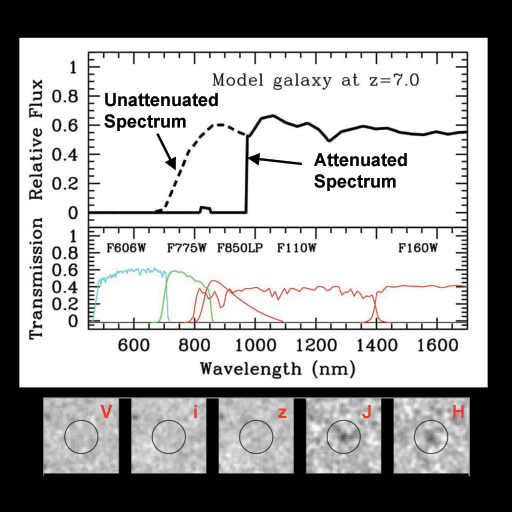
\includegraphics[width=0.5\textwidth]{../Images/drop_out_at_z7.png}
			\caption{Dropout technique for model redshift 7 galaxy\cite{first_galaxies_dropout_at_z7}.\label{fig:drop_out_at_z7}}
		\end{figure}

		The neutral hydrogen has attenuated almost all flux at wavelengths shorter than approximately 1 micrometre. The galaxy has been imaged in several different bands, and the longer wavelength filters show flux, whereas those at wavelengths corresponding to blue-ward of Lyman alpha do not. The galaxies that the group look to study have been shifted such that the drop happens in the infrared. The wavelength of the drop can be worked out using the known rest wavelength of Lyman alpha, as well as the factor by which the wavelength shifts due to the expansion of the universe, as shown in equation~\ref{eq:dropout_wavelength}.
		\begin{align}
			\text{Rest wavelength of Lyman alpha} \times (1+z) &= \text{observed wavelength of drop}\label{eq:dropout_wavelength}
		\end{align}

		Since the rest wavelength of Lyman alpha is known and the observed wavelength of the drop can be measured, the redshift of the galaxy can be determined. This
		is only a rough estimate when doing photometry since the flux is simply a number in each of the bands. For example, if the bands do not overlap, and the drop happens between two bands, it will not be known at what point the drop occurred, only the range in which it occurred. This motivates the use of bands which are close together or potentially even overlapping. Figure~\ref{fig:filter-systems} shows some different bands and their bandwidth, for different filter systems. Johnson-Cousins- Glass is one of the oldest and still the most commonly used system\cite{BasicObservationalKnowledge}.
		\begin{figure}[!htb]
			\centering
			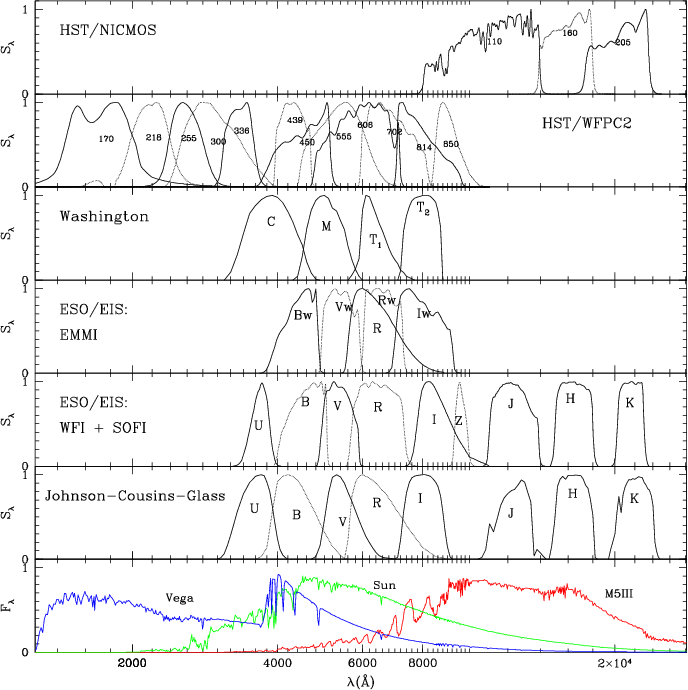
\includegraphics[width=0.65\textwidth]{../Images/filter-systems.png}
			\caption{Various filtering systems\cite{refId0}.\label{fig:filter-systems}}
		\end{figure}

		The bandwidth (or passband) is the wavelength range that can pass through the filter. Filters in different parts of the spectrum are given a common name, for example I band at \SI{806}{\nano\metre}. When observing LBGs, it is beneficial to have three filters in a row so that the position of the drop can be more accurately measured. As can be seen, there are gaps between the J H and K filters, meaning if the drop occurs between J and H, full flux should be observed in H and K and virtually no flux should be seen in J. (the panels beneath figure~\ref{fig:filter-systems} show an image (or lack thereof) of the $z=7$ galaxy in each of the V, I, z, J and H bands)

		Table~\ref{tab:filter_characteristics} below shows a list of filter names, the central wavelength of that filter, the bandwidth the filter covers, and range of redshifts for which the Lyman alpha drop would be covered. (This  range assumes the bandwidth covers 50\% either side of the central wavelength)
		\begin{table}[ht]
			\begin{center}
				\begin{tabular}{c|c|c|c}
					Filter 	& Central wavelength & Bandwidth & Redshift coverage \\
					\hline \hline
					V 	& \SI{551}{\nano\metre}	 & \SI{88}{\nano\metre} & 3.17--3.90 \\
					i 	& \SI{806}{\nano\metre}	 & \SI{149}{\nano\metre} & 5.01--7.25 \\
					Y 	& \SI{1020}{\nano\metre} & \SI{120}{\nano\metre} & 6.90--7.88 \\
					J 	& \SI{1220}{\nano\metre} & \SI{213}{\nano\metre} & 9.16--9.91 \\
					H 	& \SI{1630}{\nano\metre} & \SI{307}{\nano\metre} & 11.14--13.67 \\
					K 	& \SI{2190}{\nano\metre} & \SI{390}{\nano\metre} & 15.41--18.61
				\end{tabular}
			\end{center}
			\caption{Data highlighting which filters would be useful for observing particular redshift galaxies\cite{Galactic_Astronomy_Binney_Merrifield}}
			\label{tab:filter_characteristics}
		\end{table}

		Table~\ref{tab:filter_characteristics} must be taken into consideration that two filters should be red-ward of the drop and one blue-ward. One the fluxes have been measured in all three bands, if the object is indeed a LBG, there should be a sharp drop in flux in  one of the bands. However this does not totally rule out other possibilities: Some other objects could also exhibit a drop in flux, posing as LBGs, so usually a follow up method is used, and this is spectroscopy. Spectroscopy The drop out technique provides a good indication that a galaxy is a high redshift Lyman break galaxy, however the best way to confirm this is with spectroscopy. Spectroscopy involves\ldots

		At loads of different wavelengths, measure the spectra. Look for the drop

		Use ground based such as KECK or space based, JWST will have one.

		%JOHN IS DOING SPECTROSCOPY. I AM NOT NEEDED HERE.
		% subsection filters_and_the_dropout_technique (end)

% subsection determining_redshift (end)


    %!TEX root = mainfile.tex

\section{The Hubble Space Telescope} % (fold)
\label{sec:the_hubble_space_telescope}

	\subsection{Mission Launch} % (fold)
	\label{ssub:mission_launch}
		On April 24th 1990 NASA’s Space Shuttle Discovery launched the world’s first space-based optical telescope; The Hubble Space Telescope (HST), named in honour of American astronomer Edwin P. Hubble. Edwin Hubble’s greatest contribution to astronomy was the Hubble Law which states that galaxies are receding from us at a speed directly proportional to their distance from us. This showed that our universe is expanding, a notion which underpins modern cosmological thinking. The telescope sits in a low-Earth orbit, as shown in figure~\ref{fig:hubble_space_telescope}, at an altitude of 569 kilometres completing one orbit of the Earth every 97\,minutes\cite{Hubsite_1}.
		\begin{figure}[ht]
			\centering
			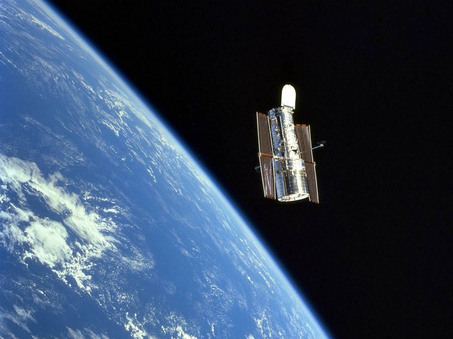
\includegraphics[width=0.5\textwidth]{../Images/Hubble_Space_Telescope.jpg}
			\caption{Photograph of HST orbiting the Earth.\label{fig:hubble_space_telescope}}
		\end{figure}

		The HST was designed to provide clear and deep views of distant galaxies and stars and most of the planets in our solar system. Hubble's domain extends from the ultraviolet through the visible and into the near-infrared\cite{NASA_1}.
	% subsection mission_launch (end)

	\subsection{Achievements to Date} % (fold)
	\label{ssub:achievements_to_date}
		The HST has provided unprecedented detail in images of star formation allowing astronomers to see the jets and disks present during the birth of new stars. It has also been able to study the atmospheric composition of extra-solar planets and take the first visible light picture of a planet outside our solar system; Fomalhaut b\cite{Hubsite_3}.

		Many EoR galaxies and candidate galaxies have been identified using HST data. In December 1995 the HST was pointed at what was believed to be a fairly empty and uninteresting patch of sky; 342 separate exposures were taken over 10 consecutive days and formed an image called the Hubble Deep Field (HDF)\cite{ESA_2}. The image contains around 3,000 objects of which the vast majority are galaxies, with a few local stars in the foreground. The HDF is one of the most iconic images of the 20th century, and it has since been cited in over 800 scientific papers.

		In 2004 its successor was revealed, the Hubble Ultra Deep Field (UDF); a million-second exposure in a 200\si{\arcsecond}$\times$200\si{\arcsecond} area of sky containing \num{10000} galaxies stretching back 13\,billion years\cite{Hubsite_2}. This exposure utilised the recently installed Advanced Camera for Surveys (ACS), seen in figure~\ref{fig:HUDF}. This survey was further refined in September 2012 in the Hubble eXtreme Deep Field (XDF) which utilised the recently installed WFC3 camera as well as combining over \num{2000} separate exposures from different sources\cite{ESA_2}.
		\begin{figure}[ht]
			\centering
			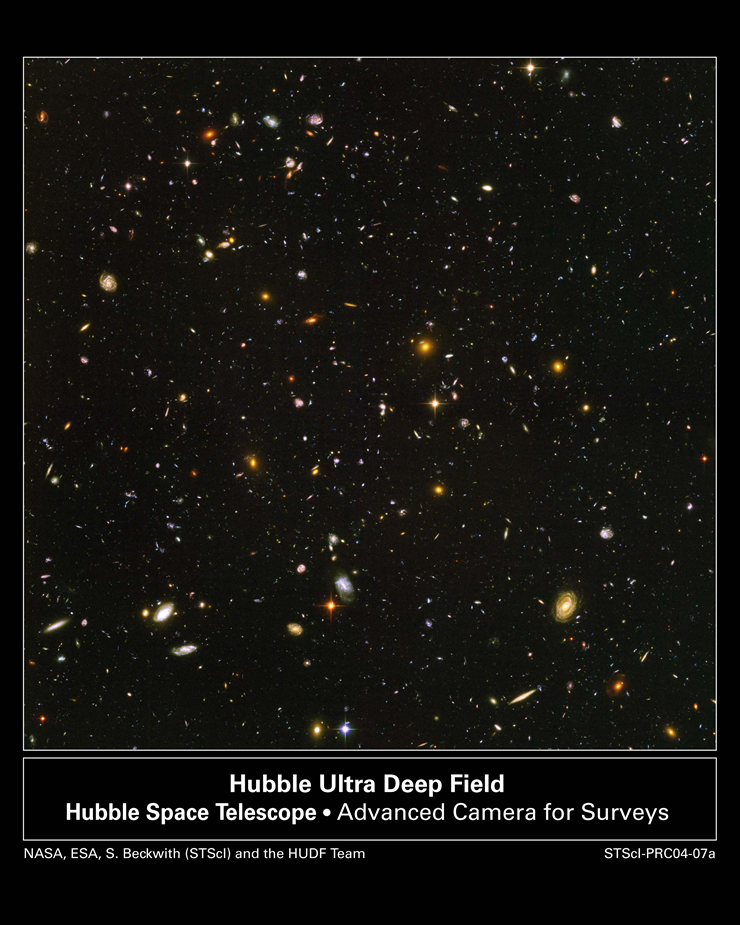
\includegraphics[width=0.8\textwidth]{../Images/HUDF.png}
			\caption{The HUbble Ultra Deep Field.\label{fig:HUDF}}
		\end{figure}

		Using data from the HUDF, object UDFj-39546284 was identified. In a paper by Bouwens et al, published in 2012, their best fit places it at a redshift of $11.8\pm0.3$\cite{Bouwens2012}. This would classify it as the oldest object ever observed. The exact nature of the object is not known but it is believed to be a mini-galaxy. Confirmation will require spectroscopic analysis, which is likely to be carried out by the James Webb Space Telescope. This observation demonstrates both the achievements and limits of the current technology.
	% subsection achievements_to_date (end)

	\subsection{Operation} % (fold)
	\label{ssub:operation}
		The HST is operated remotely from the earth, it has 4 antennae which can send and receive signals from the Flight Operations Team at Goddard Space Flight Centre in Greenbelt, Maryland via the Tracking and Data Relay Satellite system. For communication to be possible HST must have a direct line of sight to at least one of these 5 satellites.

		The HST is powered using 2 arrays of solar panels each capable of converting the Sun’s rays into \num{2800} watts of electricity. The arrays are able to store the electricity in batteries allowing the HST to remain active while in the Earth’s shadow (approximately 36\,minutes out of every 97\,minute orbit).

		Orbiting the Earth subjects the HST to extreme conditions due to the effect of zero gravity and the variation in temperature (up to around \SI{40}{\kelvin}) during each orbit. The optical system is held together using a skeleton (truss) constructed from Graphite epoxy. Graphite epoxy, commonly found in racquets and golf clubs is a stiff and lightweight material able to resist expansion and contraction due to temperature changes\cite{Hubsite_4}.
	% subsection operation (end)

	\subsection{Performance and Optical Telescope Array} % (fold)
	\label{ssub:performance_and_optical_telescope_array}
		The HST is constructed using a Ritchey-Chretien Cassegrain design; this allows high-performance over a wide field of view. The incoming light enters a tube with baffles removing any unwanted stray light, as shown in figure~\ref{fig:HST_optical_diagram} below. The light is then collected by the concave Primary mirror and reflected towards the smaller convex Secondary mirror. This light is then reflected back through a hole in the centre of the Primary mirror where it is focused onto a small area to be picked up by the instruments\cite{Hubsite_5}.
		\begin{figure}[ht]
			\centering
			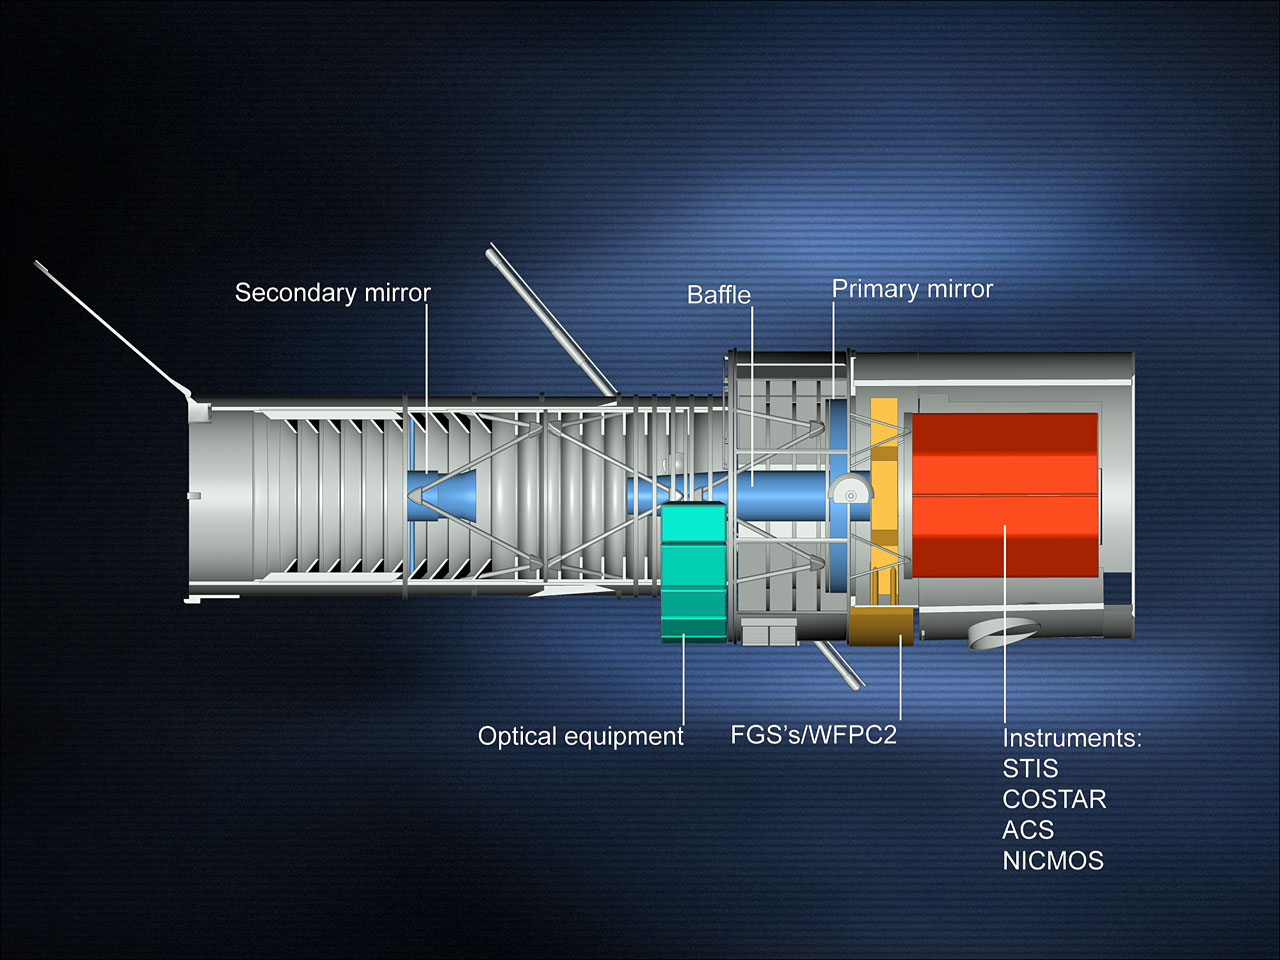
\includegraphics[width=0.5\textwidth]{../Images/HST_optical_diagram.jpg}
			\caption{Diagram showing basic systems of HST, note that WFC2 has since been replaced by WFC3.\label{fig:HST_optical_diagram}}
		\end{figure}

		The mirrors have been polished to an accuracy of better than the wavelength of visible light. When the HST was first launched the scientists soon realised that the curve to which the mirrors had been ground was not correct resulting in an error known as spherical aberration which blurred the images. A servicing mission in December 1993 deployed 5 pairs of mirrors which were able to successfully correct the error and allow Hubble to take the images it was intended to\cite{ESA_1}.

		There have been 4 servicing missions sent to the HST with the final mission taking place in May 2009. Over its lifetime the cameras and instruments have undergone many improvements and replacements. The camera currently operating that is of interest to this project is the WFC3/IR camera, installed in 2009. This camera is able to observe in the near-infra-red where we expect to see the Lyman-break galaxies. Table~\ref{tab:HST_technical} shows the key technical data for the HST, amazingly the HST is so precise it is able to lock onto a target at a distance of 1 mile without deviating more than the width of a human hair.
		\begin{table}[ht]
			\begin{center}
				\begin{tabular}{l|l}
					Component	& 	Details \\
					\hline\hline
					Primary Mirror Diameter & \SI{2.4}{\metre} \\ \hline
					Secondary Mirror Diameter & \SI{0.3}{\metre} \\ \hline
					Wavelength range & 800--1700\si{\nano\metre} \\ \hline
					Total Field of View & \SI{123}{\arcsecond}$\times$\SI{136}{\arcsecond} (\SI{16728}{\arcsecond}$^2$) \\ \hline
					Pixel Size & $18\times18$\,\si{\micro\metre} \\ \hline
					Plate Scale & \SI{0.13}{\arcsecond\per\pixel} \\ \hline
					\multirow{3}{*}{Quantum Efficiency} & 77\% at \SI{1000}{\nano\metre}\\
					 & 79\% at \SI{1400}{\nano\metre}\\
					 & 79\% at \SI{1650}{\nano\metre}\\ \hline
					Dark count &  \SI{0.048}{\electron\per\second\per\pixel} \\ \hline
					Readout noise & \SI{12.0}{\electron\per\second\per\pixel} \\ \hline
					Full Well & \SI{77900}{\electron} \\ \hline
					Gain & 2.28--2.47\si{\electron\per\ADU} \\ \hline
					Operating Temperature & \SI{145}{\kelvin} \\ \hline
					FWHM & \SI{0.151}{\arcminute} at \SI{1600}{\nano\metre}
				\end{tabular}
			\end{center}
			\caption{Technical data for HST WFC3/IR camera system\cite{WFC3_IHB}}
		\label{tab:HST_technical}
		\end{table}
	% subsection performance_and_optical_telescope_array (end)

% section the_hubble_space_telescope (end)

    %!TEX root = mainfile.tex

\subsection{Euclid} % (fold)
\label{sub:euclid}

	\subsubsection{Mission Overview} % (fold)
	\label{ssub:mission_overview}
		The Euclid mission is planned for launch in 2020, at an estimated total cost of 800\,million Euros\cite{bbc_euclid}. Its primary goal is to conduct a wide survey; some 15000 degrees of sky is planned to be covered. There is also to be a deep survey which is expected to cover around 40 degrees to a depth 2 magnitudes deeper than the wide survey. It will have a near infra-red camera and spectrometer as well as an optical camera. The primary mission  objectives are expected to be completed within 7 years. One of Euclid’s main scientific objectives with the deep field is to study high redshift galaxies at z =6+ over a very wide survey area. This will give astronomers the opportunity to spectroscopically confirm hundreds of galaxies for use in the study of the EoR. It will help constrain the bright end of the luminosity function at high z.
	% subsubsection mission_overview (end)

	\subsubsection{Capabilities} % (fold)
	\label{ssub:capabilities}
		\begin{itemize}
			\item Visual Imaging/ Photometry, 550--900\si{\nano\metre}
			\item Spectroscopy, 1100--2000\si{\nano\metre}
			\item NIR Imaging/ Photometry, 920--2000\si{\nano\metre} (Y, J,H bands)
		\end{itemize}

		Euclid will have two instruments in order to do the above; a wide-band imaging system in the visible (VIS), and an instrument capable of both slit-less spectroscopy as well as NIR imaging. These instruments will be operated simultaneously.
	% subsubsection capabilities (end)

	\subsubsection{Key Technical Data} % (fold)
	\label{ssub:key_technical_data}
		The data in table~\ref{tab:Euclid_technical} is quoted for the deep survey NIR photometry. Some data is subject to slight change as the planning stages progress.
		\begin{table}[ht]
			\begin{center}
				\begin{tabular}{l|l}
					Component & Details \\
					\hline\hline
					Primary mirror		& \SI{1.2}{\metre} \\ \hline
					FoV 				& $0.763\times0.763$\si{\degree\squared} \\ \hline
					Pixel size			& \SI{0.3}{\arcsecond}$\times$\SI{0.3}{\arcsecond} \\ \hline
					Detector Array		& \num{2000}$\times$\num{2000}\,\si{\pixel} \\ \hline
					Resolution 			& 0.3 to \SI{0.6}{\arcsecond} (in J band) \\ \hline
					Plate Scale (infra-red)	& \SI{0.3}{\arcsecond\per\pixel}
				\end{tabular}
			\end{center}
			\caption{Technical data for HST WFC3/IR camera system\cite{WFC3_IHB}.\label{tab:Euclid_technical}}
		\end{table}
	% subsubsection key_technical_data (end)
% subsection euclid (end)

    %!TEX root = mainfile.tex

\subsection{Spitzer Space Telescope} % (fold)
\label{sub:spitzer_space_telescope}
(Dorothy with contributions from Catherine)

	Spitzer Space telescope was launched by NASA on 25th August 2003\cite{fast_facts_spitzer} and is designed for use in the infrared. It was the last of NASA's ``Great Observatories'', working alongside HST in the optical, Compton Gamma Ray Observatory and Chandra X-ray Observatory. The telescope is \SI{85}{\centi\metre} in diameter, and sits in an Earth-trailing orbit around the Sun, shown in Figure~\ref{fig:spitzer_orbit_LARGE}. It is a Cassegrain telescope, meaning it has primary and secondary hyperbolic mirrors to focus the light and reduce spherical aberration, in a similar manner to Hubble. The majority of Spitzer's instrumentation is now non-operational due to a lack of cryogen, but some photometry remains possible.
	\begin{figure}[htbp]
		\centering
		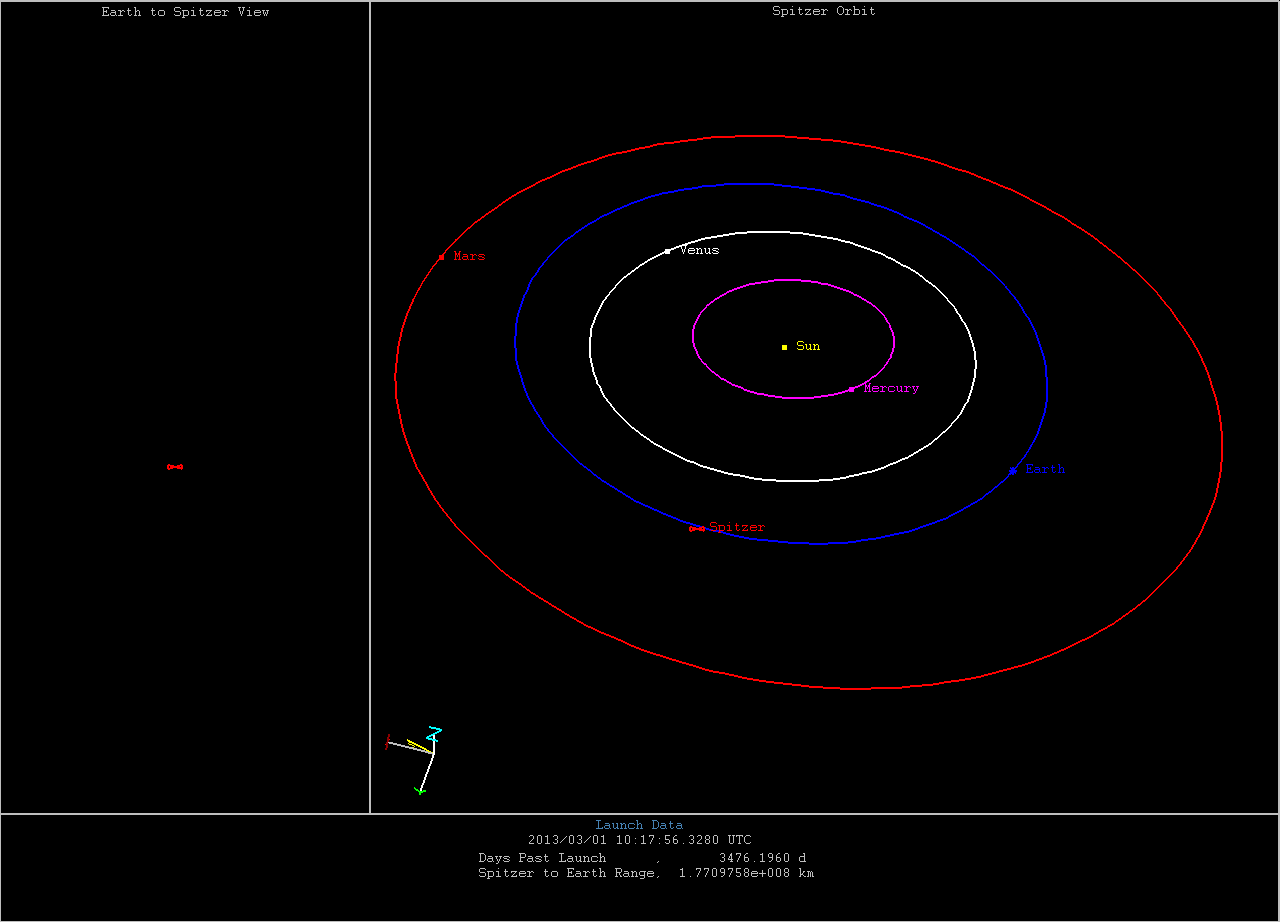
\includegraphics[trim = 110mm 70mm 5mm 30mm, clip, width=0.6\textwidth]{../Images/spitzer_orbit_LARGE.png}
		\caption{The Spitzer Space Telescope's Orbit\cite{where_is_spitzer}.\label{fig:spitzer_orbit_LARGE}}
	\end{figure}

	\subsubsection{Capabilities} % (fold)
	\label{ssub:spitzer_capabilities}
		Spitzer had the capabilities detailed in Table~\ref{tab:Spitzer_cababilities}.
		\begin{table}[htbp]
			\begin{center}
				\begin{tabular}{l|l}
					Component   &   Wavelength Range \\
					\hline\hline
					Imaging/Photometry & 3--180\si{\micro\metre} \\
					Spectroscopy       & 5--40\si{\micro\metre} \\
					Spectrophotometry  & 50--100\si{\micro\metre}
				\end{tabular}
			\end{center}
			\caption{Details of instrumentation for Spitzer\cite{WFC3_IHB}.\label{tab:Spitzer_cababilities}}
		\end{table}

		It employed three scientific instruments which helped it do the above:
		\begin{itemize}
			\item Infrared Array Camera (IRAC): an imaging camera working in the near IR at wavelengths of 3.6, 4.5, 5.8 and 8\,micrometres.
			\item Infrared Spectrograph (IRS): performing spectroscopy from 5 to 40\,micrometres.
			\item Multiband Imaging Photometer (MIPS): detected wavelengths in the far IR, at 24, 70 and 160\,micrometres.
		\end{itemize}

		The telescope was cryogenically cooled to around \SI{1.4}{\kelvin}, allowing all the instruments to function without excessive thermal interference from the telescope itself. The mission, labelled the `Cold Mission', was estimated to last between 2 and 5 years, depending on when the cryogen ran out. During this time, Spitzer imaged in all four NIR filters simultaneously, as well as doing spectroscopy, and some imaging in the far infrared. In 2009, when the cryogen ran out, the longer wavelength filters became non-operational, and the Spitzer `Warm Mission' continued imaging with the nearest IR filters ($3.6$ and $4.5$\,micrometres). This was made possible because Spitzer's orbit keeps it substantially cooler than an Earth-centred orbit would, due to the lack of IR radiation received from Earth. Furthermore it is made mostly of beryllium which has a low heat capacity at low temperatures, helping to keep it cool.

		In order to keep enough sunlight on the solar panels, Spitzer cannot point further than 120\,degrees away from the Sun. However, it also cannot get closer than 80\,degrees towards the Sun in case damage is done to the scientific instruments. This is a limitation on the area of sky which can be observed, meaning that some regions can only be seen for 40 days semi-annually, whilst other areas can be observed all year round.

		The spectrograph (IRS) operated at wavelengths too long to be of use to study the EoR, as did the far IR photometry (MIPS), however the near IR photometry capabilities of both the Spitzer warm and cold missions have been used to study high redshift galaxies, and in conjunction with HST have confirmed galaxies at redshifts as far back as $z\approx10$. Particularly the 3.6 and 4.5\,micrometre filters observe significant flux from such galaxies, and so these have been used in a number of studies looking for high redshift galaxies.
	% subsubsection capabilities (end)

	\subsubsection{Studies involving Spitzer} % (fold)
	\label{ssub:studies_involving_spitzer}
		Coe et al (2012)\cite{0004-637X-762-1-32} reports a $z\approx11$ candidate which had been observed using HST (WFC3, ACS) and Spitzer (IRAC) for longer wavelengths. This is one of the highest redshift candidates to date. The Spitzer data was taken over a total integration time of 5 hours.

		An earlier study in 2008 by Richard et al also used Hubble to detect galaxies greater than redshift seven (making use of gravitational lenses). Spitzer imaged these galaxies to help confirm that they were not foreground objects of a different nature, by looking at the flux in longer wavelength filters\cite{0004-637X-685-2-705}.

		In 2005, during the cold mission, a study was made by Spitzer on a confirmed $z=6.56$ galaxy (HCM 6A) lensed by a cluster (Abell 370). The study was used to detect the rest frame optical emission of this galaxy in order to better understand the physical properties of objects at such high redshifts\cite{1538-4357-635-1-L5}. Several other papers have also used Spitzer data in the study of high redshift galaxies.

		Spitzer also has ideal filters to look at the Balmer or \SI{4000}{\angstrom} break which, if prominent, would indicate an older stellar population and suggest that the object is more likely a contaminant than a high redshift LBG, since high redshift LBGs do not contain many old stars.

		The data in Table~\ref{tab:Spitzer_technical} shows some of the key technical data availible for the telescope.
		\begin{table}[htbp]
			\begin{center}
				\begin{tabular}{l|l}
					Component   &   Details \\
					\hline\hline
					Primary mirror & \SI{0.85}{\metre} \\
					FoV & \SI{5.2}{\arcminute}$\times$\SI{5.2}{\arcminute} \\
					Pixel size & \SI{1.2}{\arcsecond}$\times$\SI{1.2}{\arcsecond} \\
					Detector Array & $256\times256$\,\si{\pixel} \\
					\multirow{2}{*}{Full well} & 145,000 at \SI{3.6}{\micro\metre} \\
							& 140,000 at \SI{4.5}{\micro\metre} \\
				\end{tabular}
			\end{center}
			\caption{Technical data for Spitzer\cite{Spitzer_Heritage_Archive_Documentation}.\label{tab:Spitzer_technical}}
		\end{table}
	% subsubsection studies_involving_spitzer (end)
% subsection spitzer_space_telescope (end)


	%!TEX root = mainfile.tex

\section{Contaminants} % (fold)
\label{sec:contaminants}
    \subsection{Low Mass Stars} % (fold)
    \label{sub:low_mass_stars}
        These can easily be identified due to the high resolution imaging provided by \ldots. The Point-spread function (PSF) obtained will allow us to determine which sources are point-like and which are extended. We should be able to avoid significant contamination by removing any point-like sources from the results as all galaxies should have a great enough diameter.
    % subsection low_mass_stars (end)

    \subsection{Spurious Sources} % (fold)
    \label{sub:spurious_sources}
        By stipulating that we will be requiring detections in two bands the influence of spurious sources will be negligible. Finding detections in 2 bands at reasonable confidence interval (?3sig?) is very improbable. By inspecting the negative with the same requirements for detection we are able to identify any such sources easily\cite{Bouwens2011}.
    % subsection spurious_sources (end)

    \subsection{Supernovae and other transient sources} % (fold)
    \label{sub:supernovae_and_other_transient_sources}
        Events such as Supernovae happen incredibly quickly releasing a vast amount of energy, as seen in figure~\ref{fig:SNe_1987a}. These events can spoil images due to their short duration by introducing new data in only a portion of the sample. These effects are usually only considered when taking exposures years apart or when combining multiple sources over a long time scale. Such events are very unlikely to contaminate our results as we propose to take our images close in time.
        \begin{figure}[!htb]
            \centering
            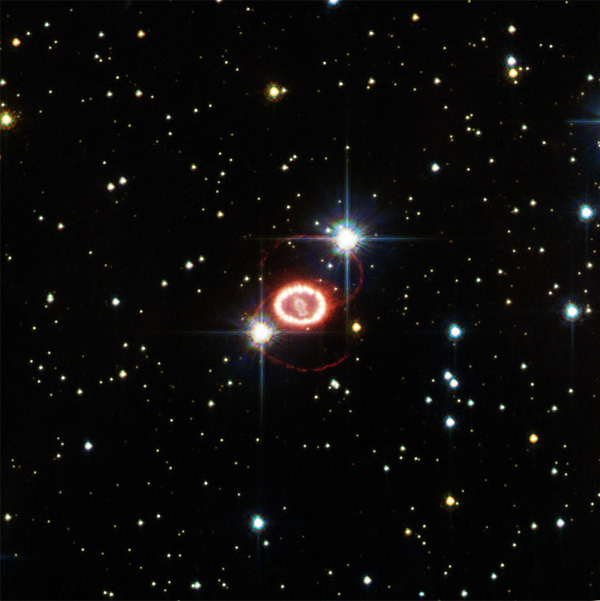
\includegraphics[width=0.6\textwidth]{../Images/SNe_1987a.jpg}
            \caption{The shock wave from Supernova 1987a imaged by HST in 2006.\label{fig:SNe_1987a}}
        \end{figure}
    % subsection supernovae_and_other_transient_sources (end)

    \subsection{Lower Redshift Sources and photometric scattering} % (fold)
    \label{sub:lower_redshift_sources_and_photometric_scattering}
        This category is likely to provide the greatest source of contamination for the surveyed area. It will do so increasingly at high redshifts where its affect on the faintest magnitudes is most greatly felt. Its affect is most influential with a small S/N ratio for the observations, by fixing this at a level of S/N = \ldots we can be confident that the contamination will be low. Detecting a source in another band such as b435, v606, i775 for YJH photometry would class it as a contaminant and then should be removed from sample.
    % subsection lower_redshift_sources_and_photometric_scattering (end)

% section contaminants (end)

% part observations (end)

\newpage
\appendix
\addcontentsline{toc}{section}{Appendix}

\section{Parameter Fit Data} % (fold)
\label{app:parameter_fit_data}

% section paramter_fit_data (end)
\newpage
\bibliographystyle{unsrt}
\bibliography{references}

\end{document}
    
